\documentclass[fleqn,10pt]{wlscirep}
\usepackage{graphicx, hyperref}
\usepackage{amsmath,amssymb} % define this before the line numbering.
\usepackage{color}

\graphicspath{{../figs/}}

\newcommand{\red}[1]{\textcolor{red}{#1}}


\title{ClassificationCam: How can optimized optics be used in optoelectronic convolutional neural networks?}
% (20 words or less)

\author[1,*]{Julie Chang}
\author[2]{Vincent Sitzmann}
\author[3]{Author Author}
\author[2]{Gordon Wetzstein}
\affil[1]{Stanford University, Bioengineering Department, Stanford, 94305, USA}
\affil[2]{Stanford University, Electrical Engineering Department, Stanford, 94305, USA}
\affil[*]{corresponding.author@email.example}

%\keywords{Keyword1, Keyword2, Keyword3}

\begin{abstract}
Example Abstract. Abstract must be under 200 words and not include subheadings or citations. Convolutional neural networks have been very successful in computer applications, but require a lot of computational effort to use. Optical computing offers inherent parallelism and can require zero power. Domain-specific cameras have shown potential to be more efficient. We combine aspects of all of these to propose a hybrid optoelectronic computational camera that uses a convolutional neural network to classify a scene. We show the potential in simulation and with optical prototype.
\end{abstract}
\begin{document}

\flushbottom
\maketitle
% * <john.hammersley@gmail.com> 2015-02-09T12:07:31.197Z:
%
%  Click the title above to edit the author information and abstract
%
\thispagestyle{empty}

\section*{Introduction}
% The Introduction section, of referenced text\cite{Figueredo:2009dg} expands on the background of the work (some overlap with the Abstract is acceptable). The introduction should not include subheadings.
\label{sec:intro}
Deep neural networks have found success in a wide variety of applications, ranging from computer vision to natural language processing to game playing \cite{lecun2015deep}. Convolutional neural networks (CNNs), capitalizing on the spatial invariance of certain properties of images, have been especially popular in computer vision problems such as image classification, image segmentation, and even image generation \cite{krizhevsky2012imagenet,goodfellow2014generative,long2015fully}. As performance on a breadth of tasks has improved to a remarkable level, the number of parameters and connections in these networks has grown dramatically, and the power and memory requirements to train and use these networks have increased correspondingly. 

% For example, the final version of Google DeepMind's AlphaGo in \cite{silver2016mastering} used 40 search threads, 48 CPUs, and 8 GPU to play a game of Go. Live imaging and sensing applications face the additional challenge of power-hungry sensors and high bandwidth transfer of data to feed into the downstream computer vision algorithms \cite{likamwa2013energy}.
While the training phase of learning parameter weights is often considered the slow stage, large models also demand significant energy during inference due to millions of repeated memory references and matrix multiplications. To increase efficiency, many strategies have been employed to compress CNNs while maintaining performance, including pruning, trained quantization, huffman encoding, and altered architectural design \cite{han2015deep,iandola2016squeezenet}. On the hardware front, there are now specialized processing units for deep learning, such as TrueNorth, Movidius's USB-based neural compute stick (NCS), and Google's tensor processing unit (TPU).  Other inference-focused efforts aimed at embedded vision applications have tried to incorporate a portion of the image processing on the sensor chip, eliminating or reducing the need to shuttle full image data to a processor \cite{gruev2002implementation,likamwa2016redeye}. Computational efficiency of CNNs continues to be an area active research, and it remains difficult for embedded systems such as mobile vision, autonomous vehicles and robots, and wireless smart sensors to deploy CNNs due to stringent constraints on power and bandwidth. 

Here we explore a complementary strategy that incorporates a layer of optical computing prior to either analog or digital electronic computing. Optical computing has been tantalizing for its high bandwidth, high interconnectivity, and inherently parallel processing, all potentially at the speed of light \cite{denz2013optical}. Certain operations can be performed in free-space or on a photonic chip with minimal to no power consumption, e.g. a lens can take a Fourier transform ``for free" \cite{yang2013chip,goodman2008introduction}.  An optimizable and scalable set of optical configurations that preserves these advantages and serves as a framework for building optical CNNs would be of interest to computer vision, robotics, machine learning, and optics communities. Initial research on optical neural networks (ONNs) was spurred by the capability of optics to perform the expensive matrix multiply of a fully connected layer \cite{farhat1985optical,psaltis1988adaptive,lu1989two,saxena1995adaptive}. Recently there has been renewed interest in ONNs both in academic research \cite{shen2017deep,bueno2017reinforcement}and in industry (Fathom Computing, Lightelligence, Optalysis). However, the ONN literature mentioned previously do not involve convolutional layers, which have become essential in computer vision applications. 

We take initial steps toward the goal of an optical CNN from a computational imaging approach, integrating image acquisition with computation via co-design of optics and algorithms. Computational cameras exploit the physical propagation of light through custom optics to encode information about a scene that would be lost in a standard 2D image capture \cite{ng2005light,levin2007image,mcguire2007optical,o2010optical,chang2016variable}. In this work, we propose a computational imaging system modeled after a feed-forward CNN that assists in performing classification of input images. By pushing one or more layers of a CNN into the optics, we reduce the workload of the electronic processor during inference. Imaging systems are often characterized by their point spread function (PSF), which describes how a single point source of light propagates through the system. For a simple linear and space-invariant system, the image recorded at the output is the convolution of the original object with the system PSF \cite{goodman2008introduction}. This built-in convolution motivated us to explore how we could use optics to perform the first convolutional layer of a CNN. The ASP Vision system previously approached the task of designing a hybrid optoelectronic CNN, using angle sensitive pixels to approximate the first convolutional layer of a typical CNN, but it is limited to a fixed set of convolution kernels \cite{chen2016asp}. Our goal is to design a system with optical elements optimized for a specific problem to demonstrate low-power inference by a custom optoelectronic CNN.

We begin by learning an optical correlator consisting of a single convolutional layer that essentially performs template matching on images, as has been explored for optical target detection and tracking \cite{gregory1986real,manzur2012optical,javidi1995optical,koppal2011wide}. Since the capabilities of a single layer linear classifier are limited, we then expand to a hybrid optoelectronic designs, in which the output of the convolutional layer is fed into a digital fully connected layer. To evaluate our designs, we build the forward model of computational light transport in a Tensorflow framework with relevant physical contraints and train these networks to perform image classification on Google QuickDraw and CIFAR-10 datasets. We use built-in backpropagation and stochastic gradient-based optimizers to learn the weights, both of the PSFs and the optical elements. We compare the simulated ONN accuracy against the unconstrained computer implementation of the same network structure. To demonstrate the validity of our simulations, we build a hybrid optoelectronic two-layer network with an optical convolutional layer and electronic fully connected layer for CIFAR-10 classification. Our proof-of-concept experiment uses bulk optics and free-space propagation, which is not necessarily practical or scalable to commercial applications. However, photonic integrated circuits could significantly help in both these regards \cite{sun2013large,rechtsman2013photonic,shen2017deep}. Combination of these next-generation large-scale photonic circuits with compressed deep learning models could provide a potential route for high performance ONNs.

% While the proposed ONN architectures offer lower power inference on classification tasks, the physical image formation imposes several constraints on the CNN architecture, including nonnegative signal and weights when using incoherent light, no bias, etc. We will discuss in more detail in the paper how much each of these constraints limit the performance of our system. 

%%%%%%%%%%%%%%%%%%%%%%%%%%%%%%%%%%%%%%%%%%%%%%%%%%%%%%%%%%%%%%%%%%%%%
%%%%%%%%%%%%%%%%%%%%%%%%%%%%%%%%%%%%%%%%%%%%%%%%%%%%%%%%%%%%%%%%%%%%%

\section*{Results}
Our primary focus in this project is to understand the potential of custom optics to implement a convolutional layer in the context of an image classification task. We first describe how this layer could be implemented, then we use this optimizable convolutional block to simulate classification models consisting either of a single optical convolutional layer (i.e. an optical correlator) or of one optical convolutional layer fed into one digital fully connected layer. Finally we present experimental results from this hybrid optoelectronic CNN prototype. Note that we assume spatially incoherent light as the input to the proposed systems as this is most relevant to an imaging scenario. We do not set out to achieve state-of-the-art classification accuracies in our toy models; rather, the goal is to distill a CNN into a few key components and evaluate whether an optical implementation can rival the electronic implementation of the analogous architecture. 

%%%=======================================%%%

\subsection*{Optical convolutional layer}

\begin{figure}[t]
\centering
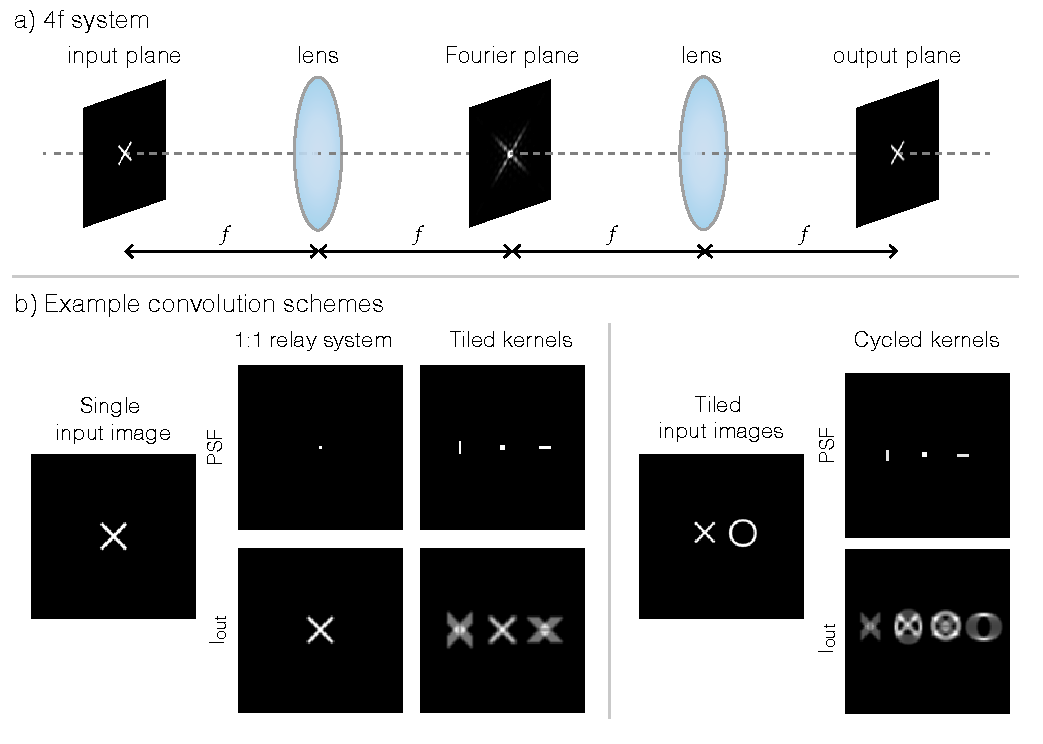
\includegraphics[width=.85\linewidth]{convolution.pdf}
\caption{a) Diagram of a 4f system that could be adapted to perform optical convolutional layers by placing a phase mask in the Fourier plane. b) Examples of convolution schemes including the input image to the 4f system, the PSF that would be formed by the phase mask, if any, in the Fourier plane, and the output image that would be formed at the output plane of the 4f system. The left panel pairs a single input image with either a single kernel or tiled kernels, and the right panel pairs tiled input images with tiled kernels, resulting in cycled kernels.}
\label{fig:convolution}
\end{figure}


A CNN typically begins with a convolutional layer, which essentially performs pattern matching with a set of learnable visual filters. A standard convolutional layer takes an input volume of depth $C_\text{in}$, performs a series of correlations with a set of $C_\text{out}$ kernels each with depth $C_\text{in}$, and outputs a new volume of depth $C_\text{out}$. The correlation of the kernel across the width and height of the input volume produces a 2D ``activation map", and stacking the $C_\text{out}$ activation maps for all kernels forms the output volume of depth $C_\text{out}$. Hyperparameters include the spatial extent of the kernel $F$, the stride with which the kernel is applied, and the padding of the input volume. Here we assume a stride of $1$, meaning the kernel is shifted by one pixel at a time, and zero-padding such that the output volume has the same height and width as the input. Each channel of the output image from a single non-strided, zero-padded convolutional layer can be described as:
\begin{equation}
I_\text{out, j}  = \sum_{i = 1}^{C_\text{in}} I_\text{in, i} \ \star \ \text{W}_{i,j}\ , \text{for } j \in 1, 2, \hdots C_\text{out} 
\end{equation}

Now let us consider how these operations may be achieved optically. In linear optical systems, image formation is often modeled as a spatially invariant convolution of the scene with the point spread function (PSF) of the system:
\begin{equation}
I_\text{out}  = I_\text{in} * \text{PSF}
\end{equation}

One way to achieve this setup is with a ``4$f$ system", a basic telescope consisting of two convex lenses performing a cascade of two Fourier transforms (Fig. \ref{fig:convolution}a). The system is so-named due to the placing of the first lens one focal distance, $f$, away from the object plane, producing a Fourier plane another distance $f$ in front of the first lens. The second lens is then placed another distance $f$ from the Fourier plane, producing a conjugate image plane a final distance $4f$ from the original object plane \ref{fig:convolution}. The Fourier plane of such a system can be modulated in amplitude and phase, akin to a bandpass filter in signal processing, which alters the PSF of the system \cite{goodman2008introduction}. This simple case can be viewed as a convolutional layer with $C_\text{in} = C_\text{out} = 1$ and the flipped PSF as the single kernel. We will also refer to the flipped PSF as the kernel since the flipping is trivial. 

\subsubsection*{Tiled kernels} Now suppose we want $C_\text{out} = n$, where $n >1$. By spatially tiling the multiple kernels as the PSF of the system in an $A \times B$ grid, the output becomes the convolution of the input image with multiple 2D kernels, but now the $n$ outputs are tiled laterally instead of stacked in depth (Fig. \ref{fig:convolution}b: ``Single input imge" + ``Tiled kernels"). Consideration can be taken to ensure these outputs are non-overlapping by adjusting the shifts $\Delta x$ and $\Delta y$, if desired. The PSF can be described as
\begin{equation}
{PSF}(x,y) = \sum_{a = 1}^{A}\sum_{b = 1}^{B} W_{aB+b} (x,y) * \delta(x - a\Delta x, y - b\Delta y),
\end{equation}
and the resulting image formation as
\begin{equation}
I_\text{out}(x,y) = [I_\text{in} * PSF](x,y) =\sum_{a = 1}^{A}\sum_{b = 1}^{B}  [I_\text{in} * W_i](x) * \delta(x - a\Delta x, y - b \Delta y)
\end{equation}
where $W$ corresponds to a standard multichannel kernel for a single channel input image. Hence we have a way to convolve a single input image with multiple 2D kernels, with the difference here being that the multiple output channels are tiled across the 2D image plane instead of stacked in a third ``depth" dimension.

\subsubsection*{Cycled kernels}
For intermediate convolutional layers, the next important extension is to incorporate $C_\text{in} = m$, where $m > 1$. If we needed to exactly imitate the digital CNN, we would need $m$ different kernels for each of the $m$ input channels. This could potentially be implemented with many of the single channel modules in parallel, with the addition of a relay that sums $m$ outputs that correspond to the different depth slices of the same kernel, but this type of setup may be prohibitively complicated to build. If we slightly relax our requirements, we could again rely on Fourier optics to perform the summation. Now suppose we have tiled input images in addition to the kernels, simplifying to 1D for now for clarity:
\begin{equation} I_\text{in}(x) = \sum_{j = 1}^m I_j(x)  * \delta(x - j\Delta x),\  PSF(x) = \sum_{i = 1}^m W_i(x)  * \delta(x - i\Delta x)\end{equation}

\begin{equation} I_\text{out} = [I_\text{in} * PSF](x)= \sum_{i=1}^n [I_\text{in} * W_i](x) * \delta(x - i\Delta x)  = \sum_{i=1}^n \sum_{j=1}^m\left( [I_\text{j} *  W_i](x) * \delta(x - j\Delta x) \right) * \delta(x - i\Delta x) 
\end{equation}
This combination of tiled images and tiled kernels results in some cycling of the kernels, but could still potentially offer enough degrees of freedom for certain tasks. An example with both tiled input images and tiled kernels is shown in Fig. \ref{fig:convolution}b: ``Tiled input images" + ``Cycled kernels".

\subsubsection*{Large PSFs} Finally, we were curious whether we even needed to think about tiling many small kernels, or rather if we could optimize for one large PSF, and leave it to the optimization to decide whether tiling was the optimal strategy. These approaches are compared in the simulations below.

\subsubsection*{Phase mask optimization} After PSF optimization, the task still remains of connecting these desired PSFs to an optical element. As mentioned earlier, the Fourier plane of a $4f$ system can be modulated with an aperture transfer function (ATF) to control the incoherent PSF of the optical relay:
\begin{equation} PSF(x,y) = |\mathcal{F}\{ATF(k_x, k_y)\}(x,y)|^2,\end{equation}
where $ k_x = \frac{x}{\lambda f}$ and $k_y = \frac{y}{\lambda f}$ denote spatial frequencies and $\lambda$ is the wavelength of light. 
The ATF is a potentially complex function that can be decomposed into amplitude and phase as $ATF = A(k_x, k_y)\cdot \exp(i \Delta \phi (k_x, k_y))$, where local amplitude $A$ can be implemented with a (usually binary) transparency mask, and phase shifts $\Delta \phi$ can be realized with a clear optical element of spatially varying thickness, which controls the optical path length and thereby phase shift induced by the element. To prevent loss of light and reduce the fabrication complexity of the ATF-defining optical element, we restrict our optimization to phase-only control. 

Given the optimized PSF(s) from the kernel weight optimization, we now want to optimize phase masks that can generate these desired PSFs:
\begin{equation} \underset{\phi}{\text{minimize}} \|PSF_\text{opt} - |\mathcal{F}\{e^{i\Delta \phi}\}|^2\|^2_\text{F}
\end{equation}
where $\|\cdot\|_\text{F}$ denotes the Frobenius norm.  Many different approaches have been taken to solve the phase retrieval problem \cite{shechtman2015phase}, but since we are already using a learning-based approach above, we can use the Tensorflow framework here as well. We initialize a random phase mask and propagate training images through the current iterate of the $4f$ system. An error is calculted against the ground truth images where the training images are convolved with the desired $PSF_\text{opt}$, and then the gradients are backpropagated to the phase masks. 

Instead of separately optimizing the PSFs and then the corresponding phase masks,  we also explored the possibility of an end-to-end optimization. To combine these steps into a single optimization problem, we implement a variant of the classification Tensorflow model where the phase mask heights were the optimizable parameter rather than the PSF weights themselves, such that the gradients of the classification error function are backpropagated all the way to the phase mask heights. 

%%%=======================================%%%

\subsection*{Simulated results}

%%
\subsubsection*{Learned optical correlator} 

For our first experiment, we simulated a classification system with a single optical convolutional layer to confirm that our proposed optical convolution layer would function as expected. The schematic of this classifier is shown in Fig. \ref{fig:correlator}a. An input image from one of $N$ classes is projected into the optical convolutional block with an optimizable PSF. The output image of the convolutional layer is partitioned into an array of $N$ sub-images corresponding to the $N$ classes, and then a score for each class was calculated by taking the maximum intensity pixel within each sub-image. The predicted class of the input image is the class with the highest score.

For these simulations, our dataset consists of images from the Google QuickDraw dataset, $N = 16$. We choose this dataset because it is slightly more complex than the MNIST handwritten digit dataset, for which a $>$90\% accuracy can be achieved with a single layer, but still relatively manageable for on optical correlator. We compare several different versions of a single convolutional layer network, beginning with the baseline of a standard multichannel convolutional layer with unconstrained weights. We use 16 channels for this convolution, which we intuitively associate with the 16 classes. Next we add in nonnegative constraints to the weights, which is necessary since the intensity of light must be nonnegative. From here we move to optically plausible 2D convolutions with only a single channel. In the third variation of Fig, \ref{fig:correlator}b, we tile 16 smaller kernels within the area of a large kernel, and finally, we remove the tiling restriction and allow for a freeform large kernel. We exclude biases and use the same number of learnable parameters in all cases. 

Averaging over five trials, we find that the multichannel cases achieve slightly higher accuracy than the single channel configurations, but the single channel 2D convolutions are still able to learn reasonable filters that achieve over 72 \% accuracy.  For a single convolutional layer, the nonnegative constraint does not negatively impact classification accuracy. Furthermore, the unconstrained large kernels performs similarly to the tiled kernels. 

Ultimately we are interested in the optical implementation of this convolutional layer, so we moved on to find the phase masks that could realize these convolutions  (Fig. \ref{fig:correlator}c). In the two-step optimization, the optimizer takes the large kernel from the kernel optimization and tries to find a phase mask that produces that exact PSF, whereas in the end-to-end optimization, the optimizer tries the find a phase mask that results in the highest classification accuracy, producing a similar PSF as a by-product. While both methods are able to produce phase masks that learn reasonable PSFs, the two-step optimization is able to achieve a higher accuracy, approaching the accuracy of the original kernels. In later phase mask optimizations, we continue separate phase mask optimization from PSF optimization.

While these results contribute to our understanding of these optical convolutional layers, an optical correlator is not powerful enough for more difficult classification tasks, for example datasets of natural images or with more categories. Furthermore, with a single layer, we still only have a linear classifier. This prompts us to add a nonlinearity and a second layer in the next set of simulations.

\begin{figure}[ht]
\centering
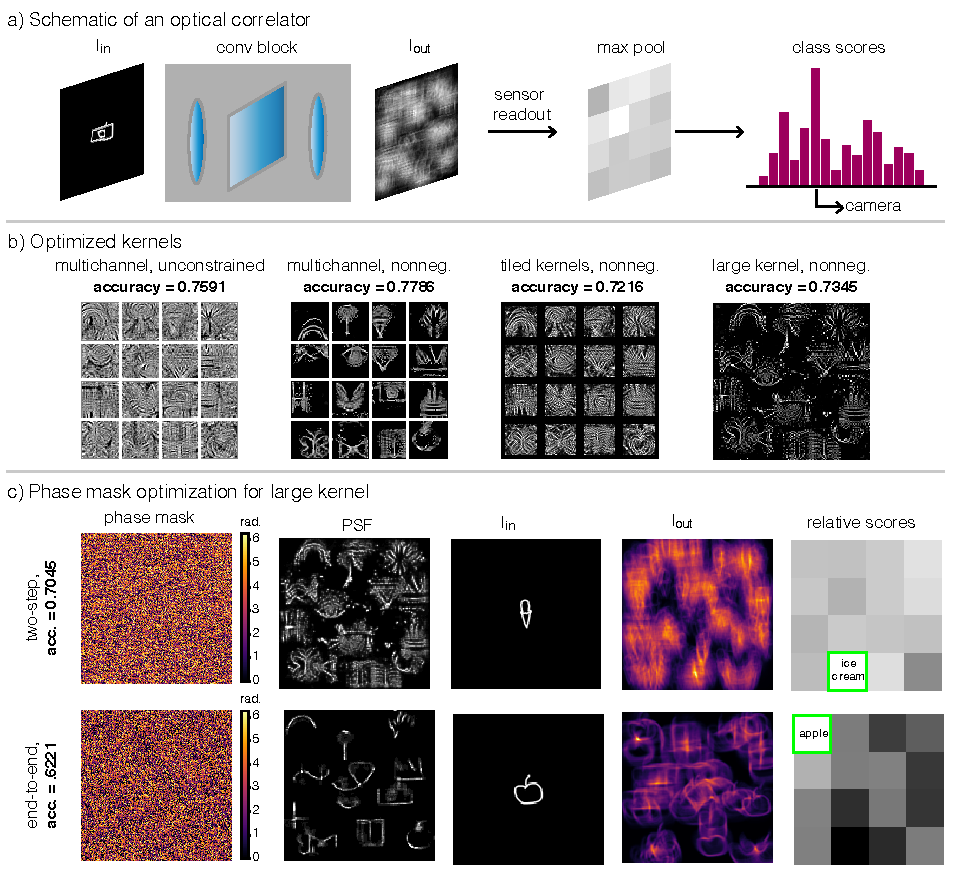
\includegraphics[width=\linewidth]{correlator.pdf}
\caption{Simulations of a learned optical correlator. a) Schematic of an optical correlator. b) Characteristic optimized kernels of a multichannel unconstrained Tensorflow convolutional layer, a multichannel nonnegative Tensorflow convolutional layer, a single channel optical convolutional layer with tiled kernels, and a single channel optical convolutional layer with a freeform large kernel. c) Optimized phase masks corresponding to the large kernel, their corresponding PSF, and an example set of input image, output image, and scores through this optical convolutional block. The top row corresponds to a two-step PSF to phase mask optimization; the bottom row corresponds to end-to-end phase mask optimization.}
\label{fig:correlator}
\end{figure}

%%
\subsubsection*{Hybrid optoelectronic CNN} 

In this set of simulations we add in two more fundamental components of a CNN: a nonlinearity and a fully connected layer. We keep the single optical convolutional layer but now process the sensor image and feed the data as input to digitally computed CNN layers (Fig. \ref{fig:hybrid}a). This allows the first layer of the CNN to be performed at zero additional power while still maintaining flexibility in the first layer weights, unlike the fixed filters of \cite{chen2016asp}. To more clearly demonstrate the performance gains with and without the zero-power optical convolutional layer, we apply this model to a more complex problem: classification of grayscale CIFAR-10 images. 

The baseline for this network architecture is an unconstrained CNN with a standard multichannel convolutional layer ($C_\text{out} = 8)$, a ReLU nonlinearity, and a fully connected layer with $N=10$ output scores. To make this optically feasible, we can tile these eight kernels across a single large kernel, spacing them sufficiently so that the eight corresponding output sub-images do not overlap. We can crop and stack the sub-images in the depth dimension, allowing for easy feeding into the rest of the Tensorflow model. This rearrangement without further constraints maintains the same performance as the baseline, since all the computations are effectively the same. However, a major limitation of a physical optical convolutional layer with incoherent light is that all the weights must be nonnegative. Exclusion of all negative weights severely limits the hypothesis space of the model (see Supplement). While this did not deterimentally impact the optical correlator, we found that once additional layers were added, nonnegative constraints resulted in significantly worse performance (Table \ref{table:hybrid}). In the nonnegative case, we normalized and shifted the sensor readout to zero-mean before feeding into the ReLU layer to ensure that the data spanned the nonlinear region. Hence, we proposed a \textit{pseudonegative} variant where half of the kernels were designated ``positive" and the other half ``negative", requiring a digital subtraction of the corresponding ``positive" and ``negative" sub-images after sensor readout, as seen in \cite{farhat1985optical}. While this requires an additional computational step, it significantly increased performance to match the unconstrained weight case.

After learning a set of pseudonegative kernels, we again run phase mask optimization to find a phase mask that can produce a PSF of tiled kernels. A sample phase mask, its corresponding PSF, and an example input-output image pair is shown in Fig. \ref{fig:hybrid}c. The ``pseudonegative" PSF after subtracting the negative half of the kernels from the positive half is shown on the bottom right, in addition to the psuedonegative images obtained after subtracting the negative half of the sub-images from the positive half. 
However, since the resultant phase mask may not produce the exact same target kernel, and the fully connected layer was originally optimized in conjunction with the target kernel, we run an additional fine-tuning optimization of the fully connected layer, keeping the phase mask fixed. The test results shown in Table \ref{table:hybrid} indicate that fine-tuning the fully connected layer after phase mask optimization is able to recover the classification accuracy back up to the non-optical-conv levels. End-to-end optimization was not successful for this model, as the solver could only find local minima in which the optical element learned to simply replicate the input image (i.e. the PSF was a single point) and the fully connected layer become responsible for all the computation (see Supplement).

Finally, we also explored the potential gains when using colored filters in our optical convolutional layer. Instead of assuming monochromatic illumination or narrow bandpass filtering, colored filters could be tiled over the sensor to effectively separate the tiled kernels into color channels. To train this version of the CNN, we used the original color RGB CIFAR-10 images. In simulation, the incorporation of color information did result in higher classification accuracy. We did not complete phase mask optimization for this case, as this would require additional attention to chromatic aberrations in a diffractive optical element, outside the scope of this paper. Nonetheless these preliminary results are promising and would be interesting to explore in the future.

\setlength{\tabcolsep}{4pt}
\begin{table}
\begin{center}
\caption{Classification accuracies on the CIFAR-10 dataset with various models. All models use grayscale images except the final ``optical conv (color)" model. Accuracies are the average of five trials.}
\label{table:hybrid}
\begin{tabular}{ l | c } 
 \textbf{Method} &  \textbf{Accuracy} \\ \hline \hline
FC only				& 0.2982	\\
conv only, unconstrained				& 0.3588	\\
conv only, nonnegative				& 0.2746	\\
conv $>$ ReLU $>$ FC, unconstrained 	& 0.5186	\\
conv $>$ ReLU $>$ FC, nonnegative	 & 0.3632	 \\
conv $>$ ReLU $>$ FC, pseudonegative & 0.5176	\\
optical conv $>$ ReLU $>$ FC, pseudonegative & 0.4142	\\
optical conv $>$ ReLU $>$ FC, pseudonegative, refined 	& 0.5096 \\ 
optical conv (color) $>$ ReLU $>$ FC, pseudonegative & 0.5770 \\
\end{tabular}
\end{center}
\end{table}
\setlength{\tabcolsep}{1.4pt}

\begin{figure}[ht]
\centering
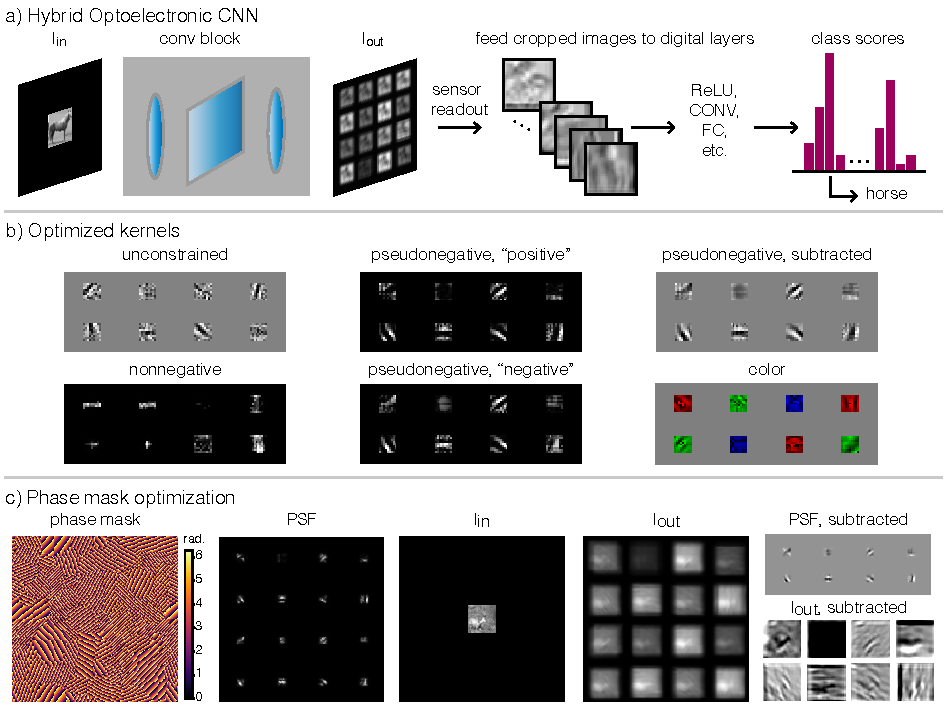
\includegraphics[width=\linewidth]{hybrid.pdf}
\caption{Simulations of a hybrid optoelectronic CNN. a) Schematic of a model with a single optical convolutional layer, after which the sensor image is processed and fed into subsequent digital CNN layers. b) On the left are characteristic optimized kernels of the convolutional layer with unconstrained weights and non-negative weights. The middle column shows the ``positive" and ``negative" half of the pseudonegative kernels. On the top right are the subtracted pseudonegative kernels. On the bottom right are the color-filtered subtracted pseudonegatve kernels, with color overlaid to indicate which channel each kernel filters. c) Optimized phase mask for monochromatic pseudonegative kernels, the corresponding PSF, a simple input-output image pais, and the subtracted kernels and sub-images.}
\label{fig:hybrid}
\end{figure}


%%%=======================================%%%

\subsection*{Experimental results}
Next we fabricated the optimized phase mask and built a prototype to test the ClassificationCam system in experiment. 

\begin{figure}[t]
\centering
% 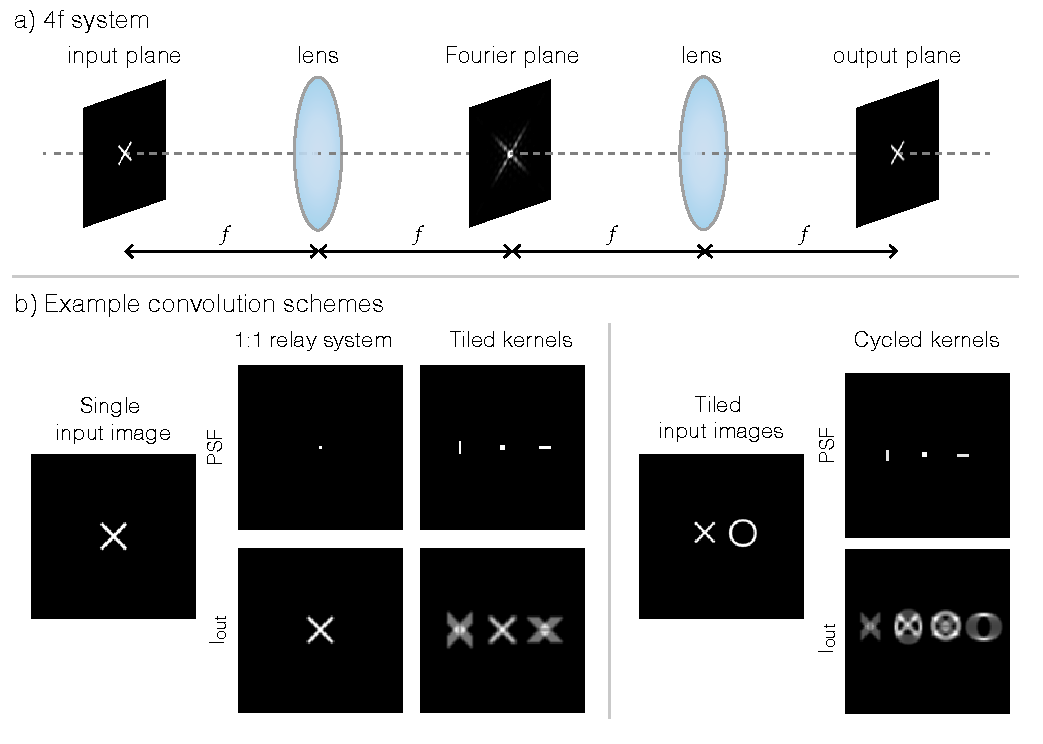
\includegraphics[width=.85\linewidth]{convolution.pdf}
\caption{Experimental results with the hybrid optoelectronic CNN.}
\label{fig:experiment}
\end{figure}

%%%%%%%%%%%%%%%%%%%%%%%%%%%%%%%%%%%%%%%%%%%%%%%%%%%%%%%%%%%%%%%%%%%%%
%%%%%%%%%%%%%%%%%%%%%%%%%%%%%%%%%%%%%%%%%%%%%%%%%%%%%%%%%%%%%%%%%%%%%

\section*{Discussion}
% The Discussion should be succinct and must not contain subheadings.
\label{sec:discussion}
Our goal here is not necessarily to match the highest accuracy achieved with a digital implementation, but rather to understand the behavior of the optical convolutional layer and assess its potential in a CNN.

Limitations
We chose to use temporally coherent light because we did not account for chromatic aberrations in the model and optimization, but this will be important to test in further studies.

single-pixel detectors (Higham2018)

potential for applications in face recognition and security

Alternatively, chromatic aberrations can be harnessed to encode color, so it would be interesting to explore multicolor masks as demonstrated in \cite{shechtman2016multicolour}.

Nonlinear operations could also be addressed optically, drawing on passive nonlinear materials or devices whose refractive indices or transmission states are dependent on optical input \cite{gibbs2012optical,christodoulides2010nonlinear}. Optical implementation could also have the potential to expand beyond traditional operations of CNNs, potentially by harnessing wave optics and quantum optics in new ways. 

Conclusion
\begin{itemize}
\item Not straightforward to generalize first optical conv. layer to multiple optical layers
\item Discuss importance of negative weights – \red{Vincent?}
\item Instead of trying to replicate a CNN exactly, could take advantage of optical transformations that aren't as practical in computations. For example, we use a 4f system for convolution, but this requires two extra lenses. Perhaps a single custom learned optical element can be used instead.
\item In the future, exploit other properties of light (polarization, phase)	
\item Specifically, coherent light and holography, photonics
\end{itemize}

%%%%%%%%%%%%%%%%%%%%%%%%%%%%%%%%%%%%%%%%%%%%%%%%%%%%%%%%%%%%%%%%%%%%%
%%%%%%%%%%%%%%%%%%%%%%%%%%%%%%%%%%%%%%%%%%%%%%%%%%%%%%%%%%%%%%%%%%%%%

\section*{Methods}
% Topical subheadings are allowed. Authors must ensure that their Methods section includes adequate experimental and characterization data necessary for others in the field to reproduce their work.
\subsection*{Datasets} 
The dataset used in the optical correlator simulation was comprised of drawings from the Google QuickDraw dataset. We used 28x28 grayscale bitmaps downloaded directly from the publically available datasets (github.com/googlecreativelab/quickdra-dataset) in 16 categories: 'apple', 'book', 'bowtie', 'butterfly', 'cake', 'camera', 'cat', 'chair', 'crown', 'diamond', 'eye', 'fish', 'hand', 'ice cream', 'lollipop', 'rainbow'. The training dataset consisted of the first 8000 images in each of the 16 categories, and the testing set the next 100 images in each category. The hybrid ONN simulation used the standard CIFAR-10 dataset \cite{krizhevsky2009learning}. For grayscale images, we took the mean over the original three color channels.

\subsection*{Network and training details}
We simulated our models in a Tensorflow framework, using built-in functions whenever possible. Since many of the kernels we tried to optimize are much larger than those of a standard CNN, we used an FFT-based convolution to increase computation speed when possible. All training was run on an Nvidia Titan X (Pascal) GPU. The various optimizations we ran can be divided into two groups: spatial domain optimization and phase mask optimization. The spatial domain optimization includes all the models that only consider the kernels and PSFs of the classification model. In these model, the inputs are images and their true category; the output is a set of scores corresponding to the possible categories. We employ a standard cross-entropy loss in these classification models, updating weights with the ADAM optimizer for 10000 iterations (learning rate = .0005). 

Phase mask optimization refers to the models where we simulate image formation through a $4f$ system with a phase mask in the Fourier plane. The height profile of the phase mask is iteratively updated until it produces a PSF that matches a target PSF, typically one produced from spatial domain optimization. The model takes sample images and target PSF as input and computes both a ground truth where the input image is convolved with a target PSF and an actual output where the input image is propagated through the current phase mask. The objective is to minimize the $\ell-2$ loss between the grount truth and model output. We run the ADAM optimizer for 50000 iterations in this case (learning rate = .0005).  The end-to-end optimizations were a special case of phase mask optimization, where the model was extended through to the final category scores. There was no predetermined target PSF for these phase masks; instead, a locally optimal PSF was produced as a byproduct of optimizing phase masks to yield a high classification accuracy. Hence for end-to-end phase mask optimization, the cross-entropy loss between the predicted scores and ground truth one-hot scores was again used.

\subsection*{Phase mask fabrication}
Phase masks were fabricated via multilayer lithography.

\subsection*{Optical setup}
532 nm laser light was scrambled through a rotating diffuser for spatial incoherence and reflected off of a binary DMD. The DMD consisted of X $\times$ X pixels that cycled through test images of the dataset. Displayed DMD images were relayed through a 4$f$ system consisting of two convex $f = 200$ mm lenses (Edmund Optics) with the custom diffractive optical element placed at the center of the Fourier plane. Output images were captured by an ORCA-Flash 4.0 sCMOS camera (Hamamatsu). Downstream processing was continued on an Nvidia Titan X (Pascal) GPU.

%%%%%%%%%%%%%%%%%%%%%%%%%%%%%%%%%%%%%%%%%%%%%%%%%%%%%%%%%%%%%%%%%%%%%
%%%%%%%%%%%%%%%%%%%%%%%%%%%%%%%%%%%%%%%%%%%%%%%%%%%%%%%%%%%%%%%%%%%%%

\bibliography{../bibliography}

\section*{Acknowledgements (not compulsory)}
% Acknowledgements should be brief, and should not include thanks to anonymous referees and editors, or effusive comments. Grant or contribution numbers may be acknowledged.
The authors would like to thank Matthew O’Toole, Donald Dansereau, and Joseph Goodman for valuable discussions. This project was supported by X.

\section*{Author contributions statement}
% Must include all authors, identified by initials, for example:
J.C, V.S, and G.W. conceived and shaped the project. J.C. and V.S. trained the models in simulation, E.P. and X.D. fabricated the custom phase masks, and J.C. conducted the experiments. J.C. wrote the manuscript, and all authors reviewed the manuscript. 

\section*{Additional information}

To include, in this order: \textbf{Accession codes} (where applicable); \textbf{Competing financial interests} (mandatory statement). 

The corresponding author is responsible for submitting a \href{http://www.nature.com/srep/policies/index.html#competing}{competing financial interests statement} on behalf of all authors of the paper. This statement must be included in the submitted article file.


\end{document}